% Body of the Week 10 study guide (study-guide.tex): every topic of the slides
% explained from scratch in a key box, followed by the exercises of that topic
% with their detailed solutions, in the order of the slides. The exercises
% are in exercises/ (one file each); \studyexercise prints the heading, the
% statement and the solution.

\maketitle

\tableofcontents
\clearpage

%======================================================================
\section{Part 1: Continuous random variables}
%======================================================================

\subsection*{Continuous random variables and their density}
\addcontentsline{toc}{subsection}{Continuous random variables and their
	density}

\begin{key}{Continuous random variables and their density}
	\setlength{\parskip}{5pt}
	\textbf{From discrete to continuous.} A discrete random variable (Week~9)
	takes finitely or countably many values, and its pmf $p(x)=P(X=x)$ gives
	each value a probability. Many quantities in finance can take
	\emph{any} value in an interval: the time until the next order, the
	fraction of a loan that is lost, a return. There are far too many values
	to give each of them a positive probability; in fact $P(X=a)=0$ for every
	single number $a$. Instead we ask for the probability of an
	\emph{interval}, and we describe it with a curve.

	\begin{minipage}[t]{.56\linewidth}
		\textbf{Density.} $X$ is \emph{continuous} if there is a function $f$,
		its \emph{density}, such that for every interval
		\[ P(a\le X\le b)=\int_a^b f(x)\,dx: \]
		the probability is the \emph{area under the curve} between $a$ and
		$b$. A density has two properties:
		\begin{enumerate}[nosep,label=(\arabic*)]
			\item $f(x)\ge0$ for every $x$ (areas are not negative);
			\item $\int_{-\infty}^{\infty}f(x)\,dx=1$ (the total area is 1,
			      because $X$ takes \emph{some} value).
		\end{enumerate}
	\end{minipage}\hfill
	\begin{minipage}[t]{.4\linewidth}
		\centering\vspace{-1mm}
		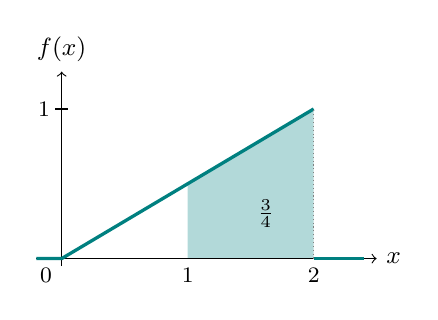
\begin{tikzpicture}[x=1.6cm,y=1.9cm,baseline=(top)]
			\coordinate (top) at (0,1.2);
			\fill[teal!30] (1,0) -- (1,.5) -- (2,1) -- (2,0) -- cycle;
			\draw[->] (-.2,0) -- (2.5,0) node[right,font=\small] {$x$};
			\draw[->] (0,-.05) -- (0,1.25) node[above,font=\small] {$f(x)$};
			\draw[very thick,teal] (-.2,0) -- (0,0) -- (2,1);
			\draw[very thick,teal] (2,0) -- (2.4,0);
			\draw[gray,densely dotted] (2,0) -- (2,1);
			\draw (-.05,1) -- (.05,1) node[left=3pt,font=\footnotesize] {$1$};
			\foreach \x in {1,2} \node[below,font=\footnotesize] at (\x,0) {\x};
			\node[below left,font=\footnotesize] at (0,0) {0};
			\node[font=\footnotesize] at (1.62,.3) {$\frac34$};
		\end{tikzpicture}
	\end{minipage}

	\textbf{Tiny example.} $f(x)=\frac x2$ for $0\le x\le2$ and $f(x)=0$
	otherwise (right). It is $\ge0$, and the total area is a triangle with
	base 2 and height 1, so it is 1. Then
	\[ P(X\le1)=\int_0^1\frac x2\,dx=\Big[\frac{x^2}{4}\Big]_0^1=\frac14,
		\qquad P(1<X\le2)=\Big[\frac{x^2}{4}\Big]_1^2=1-\frac14=\frac34. \]
	Values near 2 are more likely than values near 0: the curve is higher
	there.

	\textbf{A single point has no area.} $P(X=a)=\int_a^a f(x)\,dx=0$. So for
	a continuous $X$ it does not matter whether we write $<$ or $\le$:
	\[ P(a\le X\le b)=P(a<X<b)=P(a<X\le b)=P(a\le X<b). \]
	(For a discrete $X$ it does matter.)

	\textbf{$f(x)$ is not a probability.} It is a \emph{height}; only areas
	are probabilities. A density can be larger than 1: $f(x)=3$ on
	$[0,\frac13]$ (and 0 outside) is a density, since the area is
	$3\cdot\frac13=1$. Roughly, $P(x\le X\le x+h)\approx f(x)\,h$ for a small
	$h$: the density is probability \emph{per unit length}.

	\textbf{Finding a constant.} If $f(x)=c\,g(x)$ with an unknown $c$, use
	property (2): compute $\int g$, then $c=1/\!\int g$.
\end{key}

\studyexercise{settlement-time}

%----------------------------------------------------------------------
\subsection*{The distribution function}
\addcontentsline{toc}{subsection}{The distribution function}

\begin{key}{The distribution function}
	\setlength{\parskip}{5pt}
	\textbf{Definition.} For any random variable, discrete or continuous,
	\[ F(x)=P(X\le x)\qquad\text{for every real }x. \]
	For a continuous $X$ with density $f$ it is the area to the left of $x$,
	and the density is its derivative:
	\[ F(x)=\int_{-\infty}^{x}f(t)\,dt,\qquad f(x)=F'(x). \]
	(The second is the fundamental theorem of calculus.) So $f$ gives $F$ by
	integration, and $F$ gives $f$ by differentiation.

	\begin{minipage}[t]{.52\linewidth}
		\textbf{Probabilities from $F$.} $\{X\le b\}$ is cut into $\{X\le a\}$
		and $\{a<X\le b\}$ (for $a<b$), so
		\[ \begin{gathered} P(a<X\le b)=F(b)-F(a),\\ P(X>a)=1-F(a).
			\end{gathered} \]
		No integral is needed once $F$ is known.

		\textbf{Shape.} $F$ never decreases, it is 0 on the far left and 1 on
		the far right. For a continuous $X$ it has no jumps (a discrete $X$
		has a step function, Week~9).
	\end{minipage}\hfill
	\begin{minipage}[t]{.44\linewidth}
		\centering\vspace{-1mm}
		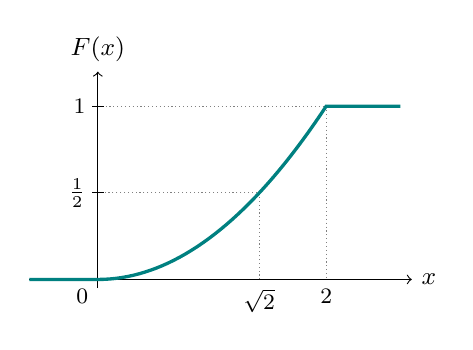
\begin{tikzpicture}[x=1.45cm,y=2.2cm,baseline=(top)]
			\coordinate (top) at (0,1.15);
			\draw[->] (-.6,0) -- (2.75,0) node[right,font=\small] {$x$};
			\draw[->] (0,-.05) -- (0,1.2) node[above,font=\small] {$F(x)$};
			\draw[gray,densely dotted] (0,1) -- (2,1) -- (2,0);
			\draw[gray,densely dotted] (1.414,0) -- (1.414,.5) -- (0,.5);
			\draw[very thick,teal] (-.6,0) -- (0,0)
			plot[domain=0:2,samples=40] (\x,{\x*\x/4}) -- (2.65,1);
			\draw (-.05,1) -- (.05,1) node[left=3pt,font=\footnotesize] {$1$};
			\draw (-.05,.5) -- (.05,.5) node[left=3pt,font=\footnotesize] {$\frac12$};
			\node[below,font=\footnotesize] at (1.414,0) {$\sqrt2$};
			\node[below,font=\footnotesize] at (2,0) {2};
			\node[below left,font=\footnotesize] at (0,0) {0};
		\end{tikzpicture}
	\end{minipage}

	\textbf{Tiny example.} The density $f(x)=\frac x2$ on $[0,2]$ from the
	previous box. For $0\le x\le2$,
	\[ F(x)=\int_0^x\frac t2\,dt=\frac{x^2}{4}, \]
	and $F(x)=0$ for $x<0$, $F(x)=1$ for $x>2$ (right). Then
	$P(X>1)=1-F(1)=\frac34$ and
	$P(0.5<X\le1)=F(1)-F(0.5)=\frac14-\frac1{16}=\frac3{16}$. Back:
	$F'(x)=\frac{2x}{4}=\frac x2=f(x)$.

	\textbf{Median.} The median is the number $m$ with $F(m)=\frac12$: $X$
	is below it with probability $\frac12$ and above it with probability
	$\frac12$. In the example $\frac{m^2}{4}=\frac12$, so
	$m=\sqrt2\approx1.414$ (only the root in $[0,2]$ counts).

	\textbf{Careful.} Write $F$ on \emph{every} part of the real line (0 on
	the left, 1 on the right), not only on the interval where $X$ lives.
\end{key}

\studyexercise{loss-given-default}

%----------------------------------------------------------------------
\subsection*{Two examples: uniform and exponential}
\addcontentsline{toc}{subsection}{Two examples: uniform and exponential}

\begin{key}{The uniform and the exponential distribution}
	\setlength{\parskip}{5pt}
	\begin{minipage}[t]{.55\linewidth}
		\textbf{Uniform on $[\alpha,\beta]$.} ``Equally likely to be anywhere
		in $[\alpha,\beta]$'': the density is constant there, and the
		constant must make the area 1,
		\[ f(x)=\frac{1}{\beta-\alpha}\ \text{ on }[\alpha,\beta],\quad 0
			\text{ outside}. \]
		The probability of a piece of $[\alpha,\beta]$ is its length divided
		by $\beta-\alpha$, so every piece of the same length is equally
		likely. For $\alpha\le x\le\beta$,
		$F(x)=\frac{x-\alpha}{\beta-\alpha}$.
	\end{minipage}\hfill
	\begin{minipage}[t]{.41\linewidth}
		\centering\vspace{-1mm}
		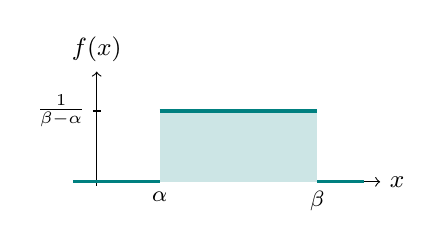
\begin{tikzpicture}[x=1cm,y=1cm,baseline=(top)]
			\coordinate (top) at (0,1.4);
			\draw[->] (-.3,0) -- (3.6,0) node[right,font=\small] {$x$};
			\draw[->] (0,-.05) -- (0,1.4) node[above,font=\small] {$f(x)$};
			\fill[teal!20] (.8,0) rectangle (2.8,.9);
			\draw[very thick,teal] (-.3,0) -- (.8,0) (.8,.9) -- (2.8,.9)
			(2.8,0) -- (3.4,0);
			\node[below,font=\footnotesize] at (.8,0) {$\alpha$};
			\node[below,font=\footnotesize] at (2.8,0) {$\beta$};
			\draw (-.05,.9) -- (.05,.9) node[left=2pt,font=\footnotesize]
			{$\frac1{\beta-\alpha}$};
		\end{tikzpicture}
	\end{minipage}

	\textbf{Tiny example.} $X$ uniform on $[0,10]$: $f(x)=\frac1{10}$ there,
	and $P(2<X<5)=\frac{5-2}{10}=0.3$, the same as $P(6<X<9)$.

	\begin{minipage}[t]{.55\linewidth}
		\textbf{Exponential with rate $\lambda>0$.} The standard model of a
		waiting time: the time until the next order, until a default, until
		a component fails.
		\[ f(x)=\lambda e^{-\lambda x}\ \text{ for }x\ge0,\quad 0\text{ for }
			x<0. \]
		For $x\ge0$,
		\[ F(x)=\int_0^x\lambda e^{-\lambda t}\,dt=\big[-e^{-\lambda t}\big]_0^x
			=1-e^{-\lambda x}, \]
		so the \emph{tail} (the chance of waiting longer than $x$) is
		$P(X>x)=e^{-\lambda x}$.
	\end{minipage}\hfill
	\begin{minipage}[t]{.41\linewidth}
		\centering\vspace{-1mm}
		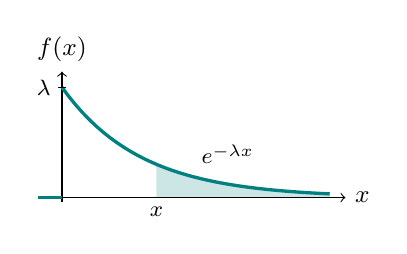
\begin{tikzpicture}[x=1cm,y=1cm,baseline=(top)]
			\coordinate (top) at (0,1.6);
			\fill[teal!20] (1.2,0) -- plot[domain=1.2:3.4,samples=30]
			(\x,{1.4*exp(-\x)}) -- (3.4,0) -- cycle;
			\draw[->] (-.3,0) -- (3.6,0) node[right,font=\small] {$x$};
			\draw[->] (0,-.05) -- (0,1.6) node[above,font=\small] {$f(x)$};
			\draw[very thick,teal] (-.3,0) -- (0,0);
			\draw[very thick,teal] plot[domain=0:3.4,samples=40]
			(\x,{1.4*exp(-\x)});
			\draw (-.05,1.4) -- (.05,1.4) node[left=2pt,font=\footnotesize]
			{$\lambda$};
			\node[below,font=\footnotesize] at (1.2,0) {$x$};
			\node[font=\footnotesize,anchor=west] at (1.65,.55) {$e^{-\lambda x}$};
		\end{tikzpicture}
	\end{minipage}

	\textbf{Tiny example.} Calls arrive at a rate of $\lambda=0.5$ per
	minute. The probability of waiting more than 2 minutes is
	$e^{-0.5\cdot2}=e^{-1}\approx0.368$, and of waiting less than 2 minutes
	$1-e^{-1}\approx0.632$.

	\textbf{Conditional probabilities.} They work as in Week~9. For $a<b$,
	the event $\{X>b\}$ is part of $\{X>a\}$, so
	\[ P(X>b\mid X>a)=\frac{P(X>b,\ X>a)}{P(X>a)}=\frac{P(X>b)}{P(X>a)}. \]
	For the exponential distribution this is
	\[ \frac{e^{-\lambda b}}{e^{-\lambda a}}=e^{-\lambda(b-a)}=P(X>b-a): \]
	having waited
	$a$ already does not change the chance of waiting $b-a$ more. The
	exponential distribution \emph{has no memory}.
\end{key}

\studyexercise{order-arrivals}

%----------------------------------------------------------------------
\subsection*{The distribution of a function of a random variable}
\addcontentsline{toc}{subsection}{The distribution of a function of a
	random variable}

\begin{key}{The distribution of a function of a random variable}
	\setlength{\parskip}{5pt}
	\textbf{The question.} We know the distribution of $X$ (for example a
	return), and we need the distribution of $Y=g(X)$ (for example the value
	$1000(1+X)$ of an investment, or $X^2$).

	\textbf{The method: first the distribution function.}
	\begin{enumerate}[nosep,label=\arabic*.]
		\item Find the possible values of $Y$.
		\item For such a $y$, write $F_Y(y)=P(Y\le y)=P(g(X)\le y)$.
		\item Rewrite the event $\{g(X)\le y\}$ as an event about $X$ alone
		      (solve the inequality for $X$), and compute its probability with
		      the distribution of $X$.
		\item If the density is needed: $f_Y(y)=F_Y'(y)$.
	\end{enumerate}

	\textbf{Linear example.} $X$ uniform on $[0,1]$, $Y=2X+3$. $Y$ lies in
	$[3,5]$, and for $3\le y\le5$
	\[ F_Y(y)=P(2X+3\le y)=P\Big(X\le\frac{y-3}{2}\Big)=\frac{y-3}{2},\qquad
		f_Y(y)=\frac12. \]
	So $Y$ is uniform on $[3,5]$: a linear function keeps the shape.

	\begin{minipage}[t]{.56\linewidth}
		\textbf{Nonlinear example.} $X$ uniform on $[0,1]$, $Y=\sqrt X$. $Y$
		lies in $[0,1]$, and for $0\le y\le1$ (right)
		\[ F_Y(y)=P(\sqrt X\le y)=P(X\le y^2)=y^2, \]
		so $f_Y(y)=2y$ on $[0,1]$. This is not constant: the square root
		pushes the values up (for example $\sqrt{0.25}=0.5$), so $Y$ is more
		likely to be near 1 than near 0. Other functions change the shape.
	\end{minipage}\hfill
	\begin{minipage}[t]{.4\linewidth}
		\centering\vspace{-1mm}
		\begin{tikzpicture}[x=3cm,y=2.4cm,baseline=(top)]
			\coordinate (top) at (0,1.12);
			\draw[->] (-.05,0) -- (1.15,0) node[right,font=\small] {$x$};
			\draw[->] (0,-.05) -- (0,1.15) node[above,font=\small] {$y$};
			\draw[very thick,teal] plot[domain=0:1,samples=60]
			(\x,{sqrt(\x)});
			\node[teal,font=\footnotesize] at (.85,1.03) {$\sqrt x$};
			\draw[gray,densely dotted] (0,.6) -- (.36,.6) -- (.36,0);
			\draw[line width=2.5pt,gold] (0,0) -- (.36,0);
			\node[left,font=\footnotesize] at (0,.6) {$y$};
			\node[below,font=\footnotesize] at (.36,0) {$y^2$};
			\node[below,font=\footnotesize] at (1,0) {1};
			\node[font=\footnotesize,align=center] at (.68,.3)
			{$\sqrt X\le y$\\ $\iff X\le y^2$};
		\end{tikzpicture}
	\end{minipage}

	\textbf{Decreasing functions flip the inequality.} If $Y=1-X$ with $X$
	uniform on $[0,1]$, then for $0\le y\le1$
	\[ F_Y(y)=P(1-X\le y)=P(X\ge1-y)=1-(1-y)=y: \]
	$Y$ is again uniform on $[0,1]$.

	\textbf{Careful.} Do not just substitute into the density: $f_Y(y)$ is
	\emph{not} simply $f_X$ evaluated at the solved-for $x$, that is, not
	$f_X\big(g^{-1}(y)\big)$. For example, for $Y=X^2$ (Exercise~\exref{square-of-uniform})
	$f_Y(y)$ is not $f_X(\sqrt y)$. Always go through $F_Y$.
\end{key}

\studyexercise{square-of-uniform}

\clearpage
%======================================================================
\section{Part 2: Joint distributions and independence}
%======================================================================

\subsection*{Joint distribution: the discrete case}
\addcontentsline{toc}{subsection}{Joint distribution: the discrete case}

\begin{key}{Joint distribution of two discrete random variables}
	\setlength{\parskip}{5pt}
	\textbf{Why two at once.} The distribution of each random variable on
	its own does not tell how they move \emph{together}: whether two stocks
	tend to rise on the same days, whether two loans tend to default
	together. For that we need their joint distribution.

	\begin{minipage}[t]{.55\linewidth}
		\textbf{Joint pmf.} For discrete $X$ and $Y$,
		\[ p(x,y)=P(X=x,\ Y=y), \]
		usually written as a table: a row for every value of $X$, a column for
		every value of $Y$. All entries are $\ge0$ and add up to 1.

		\textbf{Tiny example.} Toss a fair coin twice. $X$ = number of heads
		in the first toss, $Y$ = number of heads in both tosses. The outcomes
		TT, TH, HT, HH give $(X,Y)=(0,0),(0,1),(1,1),(1,2)$, each with
		probability $\frac14$ (right).
	\end{minipage}\hfill
	\begin{minipage}[t]{.41\linewidth}
		\centering\vspace{6mm}
		\renewcommand{\arraystretch}{1.8}\setlength{\tabcolsep}{7pt}
		\begin{tabular}{c|ccc|c}
			$X\backslash Y$ & $0$ & $1$ & $2$ & $p_X$ \\\hline
			$0$ & $\frac14$ & $\frac14$ & $0$ & $\frac12$ \\
			$1$ & $0$ & $\frac14$ & $\frac14$ & $\frac12$ \\\hline
			$p_Y$ & $\frac14$ & $\frac12$ & $\frac14$ & $1$
		\end{tabular}
	\end{minipage}

	\textbf{Marginal pmfs.} The event $\{X=x\}$ is cut into the pieces
	$\{X=x,Y=y\}$, one for each $y$, so
	\[ p_X(x)=\sum_y p(x,y)\ \ \text{(row sums)},\qquad
		p_Y(y)=\sum_x p(x,y)\ \ \text{(column sums)}. \]
	They are written in the \emph{margins} of the table, hence the name.
	Check: each marginal adds up to 1.

	\textbf{Probability of an event: add the cells.} For any event about $X$
	and $Y$, add the cells where it holds. In the example
	$P(X=Y)=p(0,0)+p(1,1)=\frac12$.

	\textbf{Joint distribution function.} For any $X$ and $Y$,
	\[ F(a,b)=P(X\le a,\ Y\le b), \]
	the sum of the cells with $x\le a$ \emph{and} $y\le b$. In the example
	$F(0,1)=p(0,0)+p(0,1)=\frac12$.

	\begin{minipage}[t]{.55\linewidth}
		\textbf{A second example.} The table on the right has
		$X,Y\in\{0,1\}$. Row sums give $p_X(0)=p_X(1)=0.5$, column sums give
		$p_Y(0)=0.4$, $p_Y(1)=0.6$, and
		$F(0,1)=p(0,0)+p(0,1)=0.3+0.2=0.5$.
	\end{minipage}\hfill
	\begin{minipage}[t]{.41\linewidth}
		\centering\vspace{2mm}
		\renewcommand{\arraystretch}{1.4}\setlength{\tabcolsep}{7pt}
		\begin{tabular}{c|cc|c}
			$X\backslash Y$ & $0$ & $1$ & $p_X$ \\\hline
			$0$ & $0.3$ & $0.2$ & $0.5$ \\
			$1$ & $0.1$ & $0.4$ & $0.5$ \\\hline
			$p_Y$ & $0.4$ & $0.6$ & $1$
		\end{tabular}
	\end{minipage}

	\textbf{Conditional probabilities} come from the table as in Week~9:
	\[ P(Y=y\mid X=x)=\frac{p(x,y)}{p_X(x)}. \]
	In the example $P(Y=2\mid X=1)=\frac{1/4}{1/2}=\frac12$, while
	$P(Y=2)=\frac14$: a head in the first toss makes two heads more likely.
\end{key}

\studyexercise{two-stocks}

%----------------------------------------------------------------------
\subsection*{Joint distribution: the continuous case}
\addcontentsline{toc}{subsection}{Joint distribution: the continuous case}

\begin{key}{Joint density of two continuous random variables}
	\setlength{\parskip}{5pt}
	\textbf{Joint density.} The pair $(X,Y)$ is a random point of the plane.
	A \emph{joint density} is a function $f(x,y)\ge0$ such that for every
	region $A$ of the plane
	\[ P\big((X,Y)\in A\big)=\iint_A f(x,y)\,dx\,dy, \]
	and the total is $\iint f=1$. In one variable a probability was the
	\emph{area} under a curve; now it is the \emph{volume} under the surface
	$f$, above the region $A$.

	\textbf{Double integrals.} Integrate in two steps: the inner integral
	first (with the other variable held fixed, like a constant), then the
	outer one. On a rectangle both bounds are numbers; on a region like
	$\{y<x\}$ the inner bounds depend on the outer variable.

	\textbf{Marginal densities: integrate the other variable out.}
	\[ f_X(x)=\int_{-\infty}^{\infty}f(x,y)\,dy,\qquad
		f_Y(y)=\int_{-\infty}^{\infty}f(x,y)\,dx. \]
	(The continuous version of the row and column sums.) The joint
	distribution function is
	\[ F(a,b)=P(X\le a,\ Y\le b)=\int_{-\infty}^{a}\!\int_{-\infty}^{b}
		f(x,y)\,dy\,dx. \]

	\textbf{Tiny example.} $f(x,y)=6xy^2$ on the unit square $0\le x\le1$,
	$0\le y\le1$, and 0 elsewhere. The total is 1 (inner integral over $y$
	first):
	\[ \int_0^1\!\!\int_0^1 6xy^2\,dy\,dx=\int_0^1 6x\cdot\frac13\,dx
		=\int_0^1 2x\,dx=1. \]
	The marginals, and the joint distribution function at
	$\big(\frac12,\frac12\big)$:
	\[ f_X(x)=\int_0^1 6xy^2\,dy=2x,\qquad f_Y(y)=\int_0^1 6xy^2\,dx=3y^2
		\qquad(\text{on }[0,1]), \]
	\[ F\Big(\frac12,\frac12\Big)=\int_0^{1/2}\!\!\int_0^{1/2}6xy^2\,dy\,dx
		=6\cdot\Big[\frac{x^2}{2}\Big]_0^{1/2}\cdot\Big[\frac{y^3}{3}\Big]_0^{1/2}
		=6\cdot\frac18\cdot\frac1{24}=\frac1{32}. \]

	\begin{minipage}[t]{.6\linewidth}
		\textbf{A region that is not a rectangle.} $P(X>Y)$ is the volume
		above the triangle $\{0\le y<x\le1\}$ (right, dark). For a fixed $x$,
		$y$ runs from 0 to $x$ (the gold segment), and then $x$ runs from 0
		to 1:
		\[ \begin{aligned}
				P(X>Y) & =\int_0^1\!\Big(\int_0^x 6xy^2\,dy\Big)dx
				=\int_0^1 6x\cdot\frac{x^3}{3}\,dx \\
				       & =\int_0^1 2x^4\,dx=\frac25.
			\end{aligned} \]
	\end{minipage}\hfill
	\begin{minipage}[t]{.36\linewidth}
		\centering\vspace{-1mm}
		\begin{tikzpicture}[scale=2,baseline=(top)]
			\coordinate (top) at (0,1.1);
			\fill[teal!12] (0,0) rectangle (1,1);
			\fill[teal!45] (0,0) -- (1,0) -- (1,1) -- cycle;
			\draw[->] (-.08,0) -- (1.25,0) node[right,font=\small] {$x$};
			\draw[->] (0,-.08) -- (0,1.25) node[above,font=\small] {$y$};
			\draw[thick,navy] (0,0) rectangle (1,1);
			\draw[gray,dashed] (0,0) -- (1,1);
			\draw[gold,line width=1.5pt] (.55,0) -- (.55,.55);
			\node[below,font=\footnotesize] at (1,0) {1};
			\node[left,font=\footnotesize] at (0,1) {1};
			\node[below,font=\footnotesize] at (.55,0) {$x$};
			\node[font=\footnotesize] at (.8,.14) {$y<x$};
			\node[font=\footnotesize] at (.3,.75) {$y>x$};
		\end{tikzpicture}
	\end{minipage}

	\textbf{Careful.} Draw the region first, and read the bounds of the inner
	integral from the picture.
\end{key}

\studyexercise{joint-density-square}

%----------------------------------------------------------------------
\subsection*{Independent random variables}
\addcontentsline{toc}{subsection}{Independent random variables}

\begin{key}{Independent random variables}
	\setlength{\parskip}{5pt}
	\textbf{Definition.} $X$ and $Y$ are \emph{independent} if every event
	about $X$ is independent of every event about $Y$ (independent events,
	Week~9): for all sets $A$, $B$,
	\[ P(X\in A,\ Y\in B)=P(X\in A)\,P(Y\in B), \]
	equivalently $F(a,b)=F_X(a)\,F_Y(b)$ for all $a$, $b$. In words: knowing
	the value of $X$ does not change the distribution of $Y$.

	\textbf{Discrete check.} $p(x,y)=p_X(x)\,p_Y(y)$ for \emph{every} cell of
	the table. One cell that fails is enough for ``not independent''. In the
	coin example of the discrete box,
	$p(0,0)=\frac14$ but $p_X(0)\,p_Y(0)=\frac12\cdot\frac14=\frac18$, so $X$
	and $Y$ are not independent (no surprise: $Y$ counts the first toss
	too). Note that $p(0,1)=\frac14=\frac12\cdot\frac12$ \emph{does} hold;
	one good cell proves nothing.

	\textbf{Continuous check.} $f(x,y)=f_X(x)\,f_Y(y)$ for all $x$, $y$. In
	practice: if the density is positive on a rectangle (or on the whole
	quadrant) and splits there into a function of $x$ times a function of
	$y$, then $X$ and $Y$ are independent. In the example of the continuous
	box, $X$ and $Y$ are independent, and the distribution functions agree:
	\[ 6xy^2=2x\cdot3y^2=f_X(x)\,f_Y(y),\qquad
		F\big(\tfrac12,\tfrac12\big)=\tfrac1{32}
		=\tfrac14\cdot\tfrac18=F_X\big(\tfrac12\big)F_Y\big(\tfrac12\big). \]
	\textbf{Careful:} if the density is positive only on a triangle such as
	$\{0<y<x<1\}$, $X$ and $Y$ are \emph{not} independent, even if $f$ is
	constant there: knowing $X=0.1$ forces $Y<0.1$.

	\textbf{Using independence.} If $X$ and $Y$ are independent and we know
	the marginals, the joint distribution is their product, and
	probabilities of ``and'' multiply. Example: two independent waiting
	times, exponential with rates $\lambda$ and $\mu$. Both are longer than
	$t$ with probability
	\[ P(X>t,\ Y>t)=P(X>t)\,P(Y>t)=e^{-\lambda t}e^{-\mu t}
		=e^{-(\lambda+\mu)t}, \]
	and ``at least one is at most $t$'' is the complement,
	$1-e^{-(\lambda+\mu)t}$.

	\textbf{Same marginals, different joint.} Two pairs can have the same
	marginals but different joint distributions: the marginals alone do not
	tell how $X$ and $Y$ move together. For example, with $X,Y\in\{0,1\}$,
	the tables with cells $p(0,0)=p(1,1)=\frac12$, $p(0,1)=p(1,0)=0$ and with
	all four cells $\frac14$ both have marginals $\frac12,\frac12$; in the
	first $P(X=Y)=1$, in the second $P(X=Y)=\frac12$. Independence is just
	one possible joint distribution. Exercise~\exref{two-stocks-independence}
	does the same for the two stocks.
\end{key}

\studyexercise{two-stocks-independence}
\studyexercise{two-default-times}

%----------------------------------------------------------------------
\subsection*{More practice}
\addcontentsline{toc}{subsection}{More practice}

The exercises of this week are numbered by topic, so the numbers missing
above are further exercises on the same topics. They are for self-study:
you find them on the Exercises page of this week on the course website, each
with a detailed solution.
\begin{center}
	\renewcommand{\arraystretch}{1.15}
	\begin{tabular}{ll}
		\toprule
		Topic                                    & Exercises for self-study                                \\\midrule
		Continuous random variables and density  & \exref{power-density}--\exref{waiting-for-the-bus}      \\
		Distribution function                    & \exref{recovery-rate}, \exref{from-cdf-to-density}      \\
		Uniform and exponential                  & \exref{service-calls}, \exref{default-time}             \\
		Function of a random variable            & \exref{portfolio-value}--\exref{log-of-uniform}         \\
		Joint distribution, discrete             & \exref{three-coins}, \exref{insurance-claims}           \\
		Joint distribution, continuous           & \exref{exponential-pair}, \exref{triangle-density}      \\
		Independent random variables             & \exref{meeting-time}, \exref{which-are-independent}     \\\bottomrule
	\end{tabular}
\end{center}
